\chapter{Guida Cliente}
\label{app:cliente}
Il cliente visita il sito all'indirizzo \url{http://www.avifauna.fem2ambiente.com} e a partire dalla homepage (figura~\ref{fig:cl-homepage-wp}) può navigare nel sito espositivo (costruito sfruttando {\wp}) fino a quando non accede alla sezione \textsf{Ordini} del Portale Avifauna cliccando sull'apposito bottone nella barra di navigazione.

Come mostrato nello schema~\ref{fig:flusso-cliente} della relazione il flusso cliente è molto schematico, e principalmente può dividersi in \textsf{Registrato} o \textsf{Non Registrato}.

\begin{figure}
 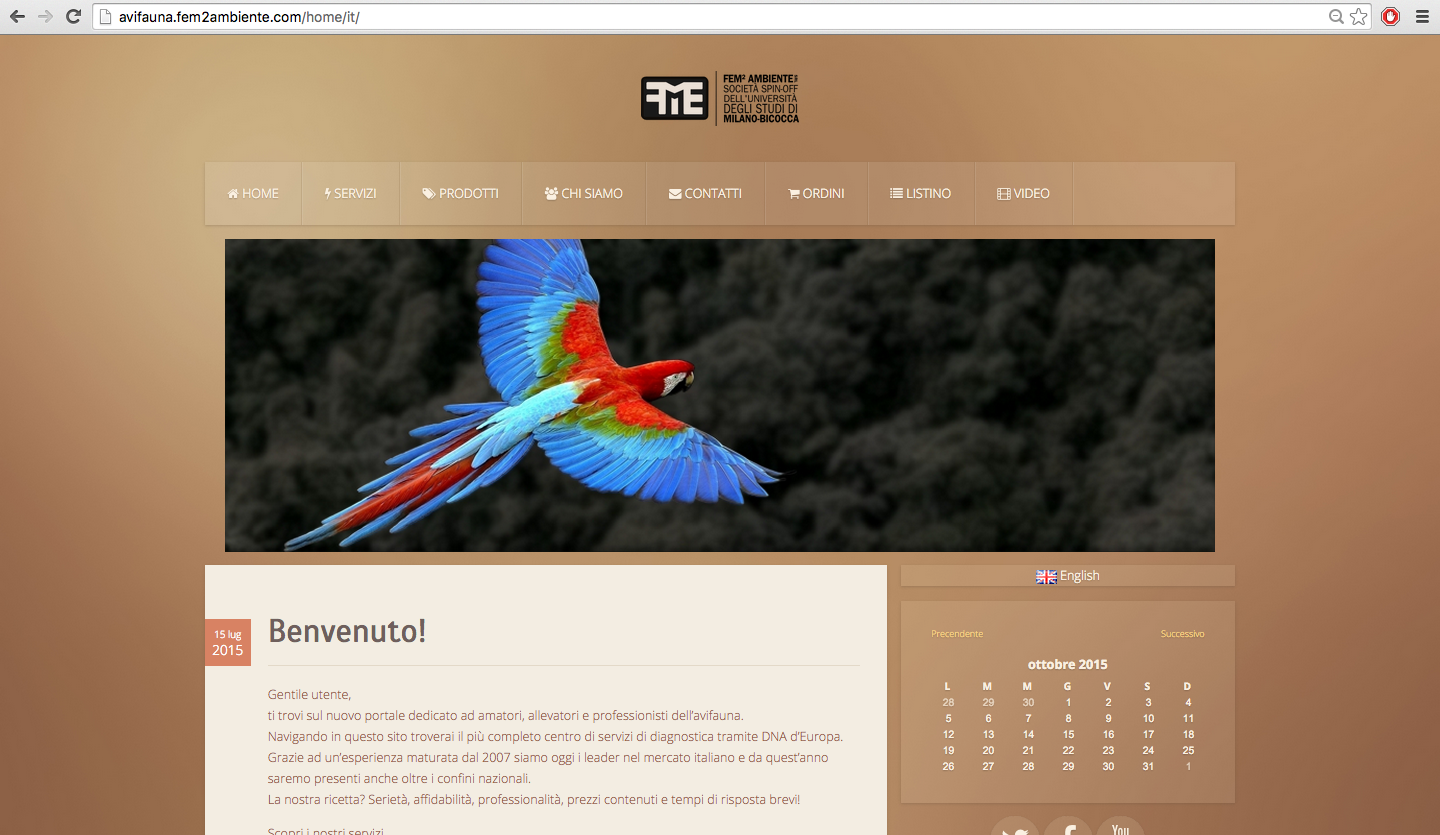
\includegraphics[width=0.95\textwidth]{images/cl-homepage-wp} 
 \caption{homepage del Portale per la Diagnostica Molecolare Avifauna}
 \label{fig:cl-homepage-wp}
\end{figure}

\section*{Registrazione}
Il cliente \textsf{Non Registrato} al momento dell'accesso alla piattaforma ordini viene indirizzato alla procedura di registrazione (figura~\ref{fig:cl-homepage-p}).

Nella pagina di \textsf{Registrazione} (figura~\ref{fig:cl-registrazione}) è necessario compilare in maniera opportuna tutti i campi richiesti ed indicati come obbligatori, accettare i termini e condizioni d'uso e procedere con la registrazione. Il sistema genera un messaggio di posta elettronica spedito all'indirizzo e-mail inserito in sede di registrazione, nel quale si trova un link di conferma. Navigando fino al link inserito nella mail il cliente accede alla propria \textsf{Pagina Personale}.

\begin{figure}
 \centering
 \begin{subfigure}[b]{0.75\textwidth}
   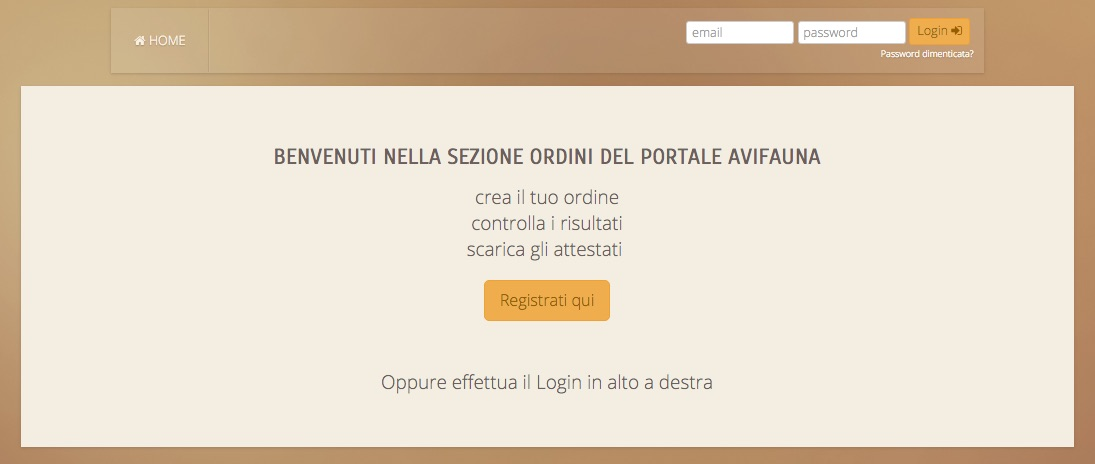
\includegraphics[width=\textwidth]{images/cl-homepage-p}
   \caption{homepage piattaforma ordini}
   \label{fig:cl-homepage-p}
 \end{subfigure}
 \begin{subfigure}[b]{0.6\textwidth}
   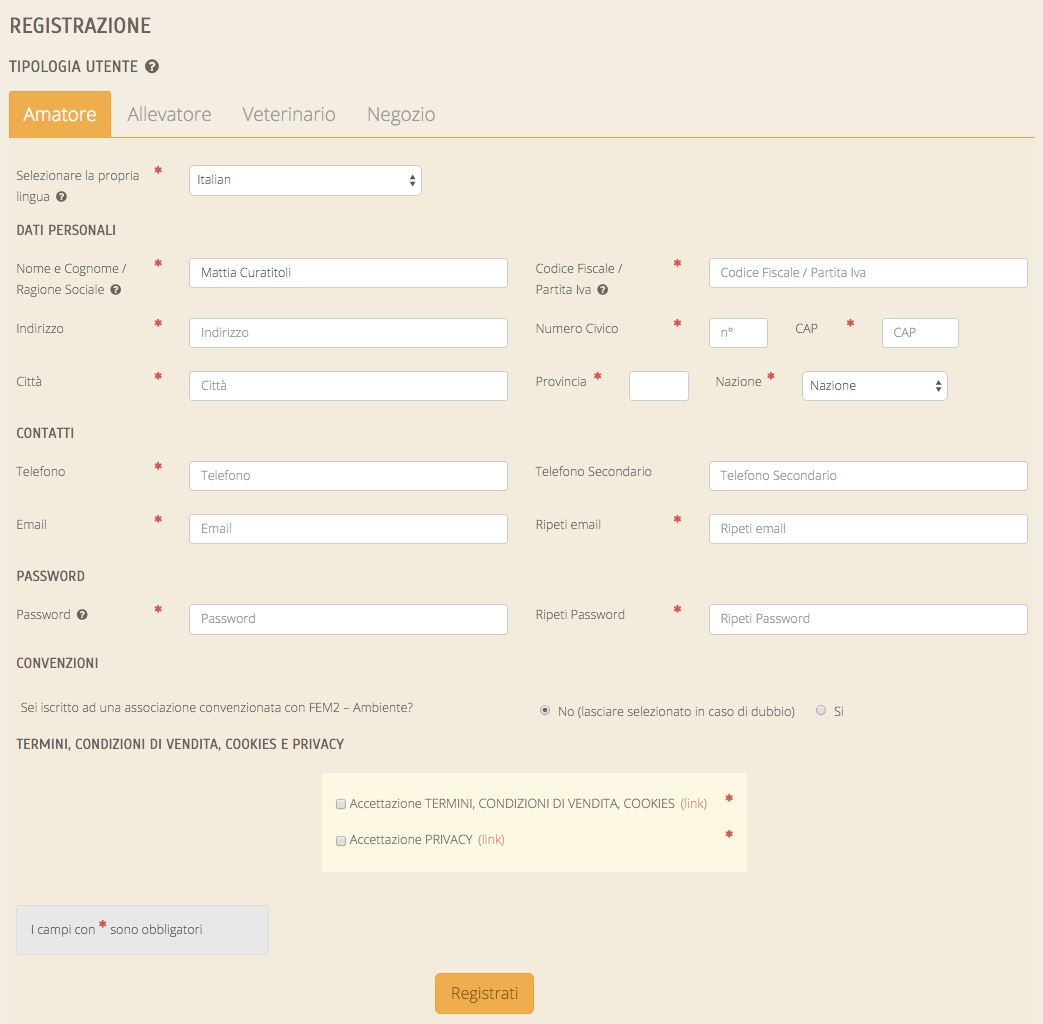
\includegraphics[width=\textwidth]{images/cl-registrazione} 
   \caption{pagina di registrazione}
   \label{fig:cl-registrazione}
 \end{subfigure}
 \begin{subfigure}[b]{0.75\textwidth}
   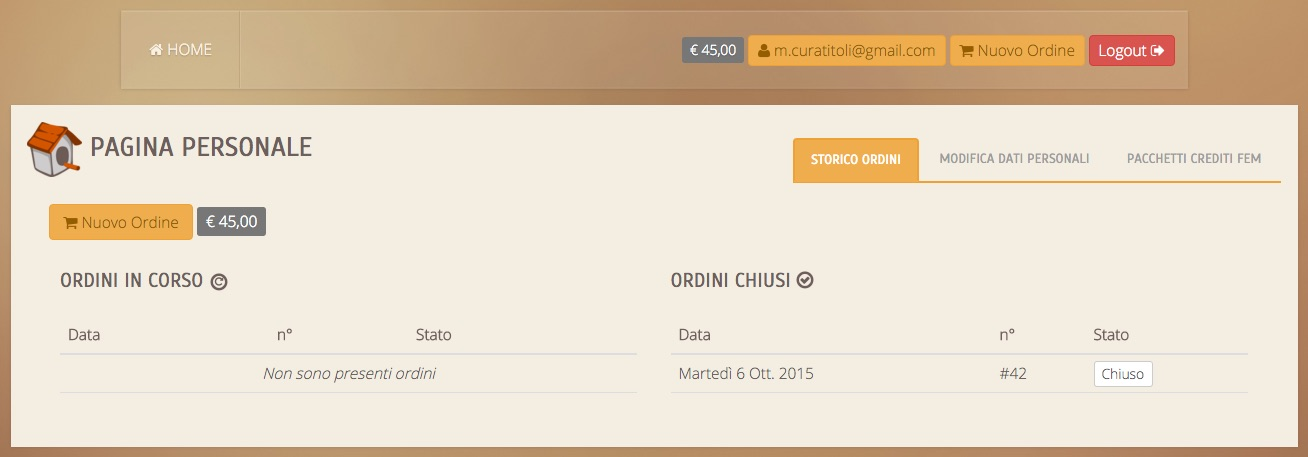
\includegraphics[width=\textwidth]{images/cl-pagina-personale}
   \caption{pagina personale del cliente}
   \label{fig:cl-pagina-personale} 
 \end{subfigure}
 \caption{flusso di registrazione cliente}
\end{figure}

\section*{Pagina Personale}
Il cliente \textsf{Registrato} invece può inserire le proprie credenziali nel form di login per accedere alla propria \textsf{Pagina Personale} (figura~\ref{fig:cl-pagina-personale}).

Effettuando il \textsf{logout} si trova nella homepage della piattaforma ordini descritta in precedenza.

La pagina personale è divisa in tre sezioni: 
\begin{itemize}
 \item lo \textsf{storico ordini} in sui vengono elencati e mostrati gli ordini in corso e quelli chiusi;
 \item la \textsf{modifica dati personali} in cui il cliente può modificare i propri dati come l'indirizzo di spedizione, la lingua preferita o la password;
 \item l'acquisto \textsf{pacchetti crediti FEM} in cui vengono visualizzati gli acquisti di pacchetti crediti effettuati ed è possibile acquistarne di nuovi.
\end{itemize}

La pagina personale è costruita per mostrare al cliente tutte le informazioni essenziali, come i crediti posseduti, il proprio nome utente (indirizzo e-mail) e, come sezione principale, lo storico degli ordini sottoforma di due tabelle.

La sezione per la modifica dei dati personali è essenzialmente un form analogo a quello di registrazione in cui vengono mostrati i dati personali inseriti e si fornisce la possibilità di modificarli.

Per acquistare pacchetti crediti FEM invece si deve accedere alla sezione apposita attraverso un tasto in alto a destra, in cui mostrata la cronologia delle transazione relativi agli acquisti di crediti (in modo da indicare la data e le coordinate per il pagamento in caso in cui non fosse stato ancora eseguito), dopodichè si può attraverso un apposito form selezionare la modalità di pagamento preferita e la quantità di crediti da acquistare tra le possibilità proposte in un menù a tendina.

Dalla pagina personale si può anche creare un \textsf{Nuovo ordine} cliccando sul tasto apposito.

\section*{Nuovo Ordine}
La pagina dedicata alla creazione di un nuovo ordine si divide in 3 blocchi principali: \textsf{carrello}, \textsf{riepilogo} e \textsf{pagamento}, più un eventuale fase di \textsf{attesa} in caso di campioni con specie non presente nell'elenco fornito da {\fem} (struttura rappresentata dallo schema~\ref{fig:nuovo-ordine-s}).

Nel \textsf{carrello} viene mostrata una tabella in cui vengono aggiunti man mano i campioni da analizzare con tutte le informazioni correlate. Più in basso si trova il form per l'inserimento del singolo campione, che richiede informazioni obbligatorie come l'identificativo, la specie, la spunta ad almeno un analisi, e opzionali come la mutazione o il nominativo del proprietario del soggetto (figura~\ref{fig:cl-nuovo-ordine-carrello}).

Particolare è l'inserimento della specie che al momento della scelta fa comparire un box a lato (o sotto in caso di visita del sito attraverso dispositivo mobile) con immagine e informazioni aggiuntive relative alla specie e sottospecie scelta. Se la specie non è presente nell'elenco si può inserire in un campo testuale il nome indicante la specie desiderata.

Al momento della scelta dell'analisi è possibile spuntare esclusivamente le checkbox per gli attestati (cartaceo e digitale) relativi all'analisi selezionata. Inoltre in un box colorato a fianco sono elencate le analisi scelte, con i relativi costi, e i consigli per usufruire di sconti.

Cliccando il tasto \texttt{inserimento campione} si va ad aggiungere il campione alla tabella del carrello.

Per procedere si avanza nella sezione del \textsf{riepilogo} (figura~\ref{fig:cl-nuovo-ordine-riepilogo}) in cui è riproposto l'elenco di soggetti da analizzare, il prezzo di ognuno e gli attestati da spedire. In caso di campioni di specie \emph{junior} o specie definita \emph{RNS} compare sotto alla tabella un form per l'inserimento dei cosiddetti \emph{standard} (figura~\ref{fig:cl-nuovo-ordine-r-standard}).

Come spiegato nel capitolo~\ref{subs:specie} della relazione, alcune sottospecie sono denominate \emph{junior} in quanto {\fem} non ha ancora acquisito un'esperienza minima per la quale assicurare il totale successo e veridicità delle analisi effettuate. Per avere più indicazioni e precisione vengono richiesti (se a disposizione del cliente) gli \emph{standard}, ovvero campioni di soggetti il cui sesso è già noto (la caratteristica junior si applica solo in caso di analisi riguardante il sesso), tipicamente i genitori, in modo tale da avere alcuni riferimenti in più.

Le specie \emph{RNS} sono invece quelle specie inserite nel campo testuale perché non trovate nell'elenco proposto da {\fem}; queste specie sono considerate nuove, quindi da valutare dagli tecnici dell'azienda, e richiedono anch'essi eventuali standard per avere maggiori riferimenti. Come mostrato nello schema del flusso ordini~\ref{fig:flusso-ordine} le richieste RNS allungano il processo di creazione dell'ordine. In questi casi infatti prima della scelta del pagamento l'ordine viene arrestato e messo in stato di \textsf{attesa gestione da parte dei tecnici FEM} (figura~\ref{fig:cl-nuovo-ordine-attesa}).

Un addetto dell'azienda riceverà una notifica e si occuperà della situazione: alcune volte capita di dover aggiungere all'elenco la specie inserita dal cliente, molto più spesso si è trattato di una svista, quindi verrà corretta la specie inserita con quella corretta già presente nel database.

A seguito di questa gestione lo stato dell'ordine avanza e avvisa il cliente che l'ordine è pronto per essere pagato.

Si arriva così all'ultimo dei tre blocchi, ovvero il \textsf{pagamento} in cui viene calcolato il totale della spesa e si può scegliere la modalità di pagamento scelta tra una lista di proposte (figura~\ref{fig:cl-nuovo-ordine-pagamento}).

\begin{figure}
 \centering
 \begin{subfigure}[b]{0.32\textwidth}
   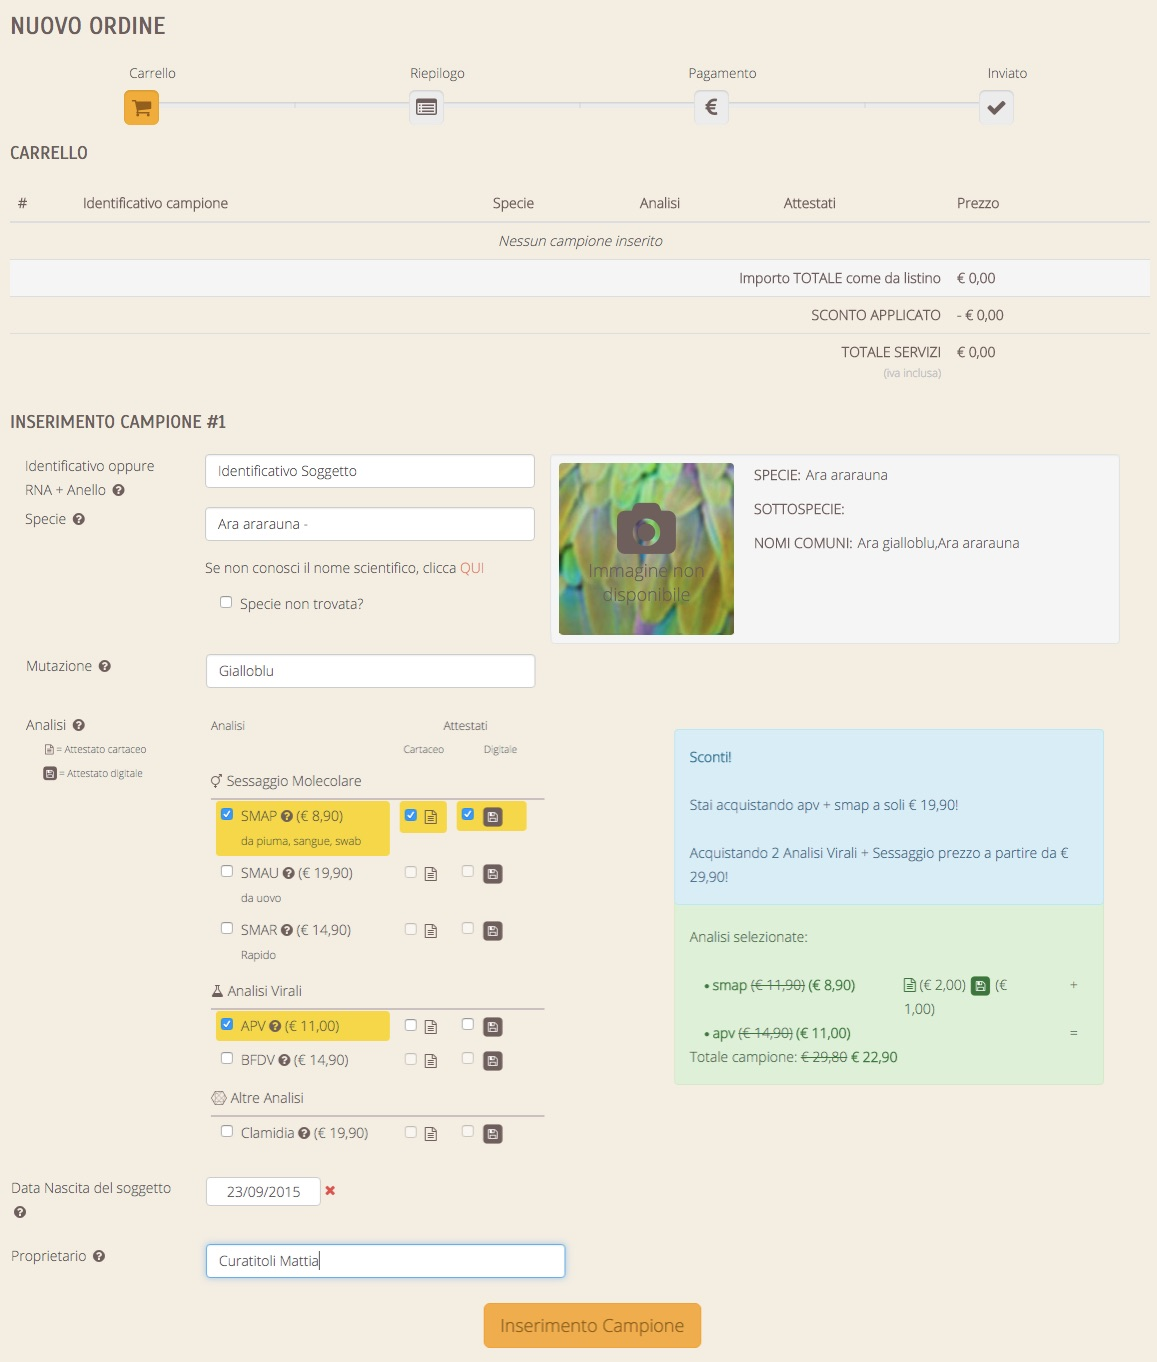
\includegraphics[width=\textwidth]{images/cl-nuovo-ordine-carrello}
   \caption{carrello}
   \label{fig:cl-nuovo-ordine-carrello}
 \end{subfigure}
 \begin{subfigure}[b]{0.33\textwidth}
   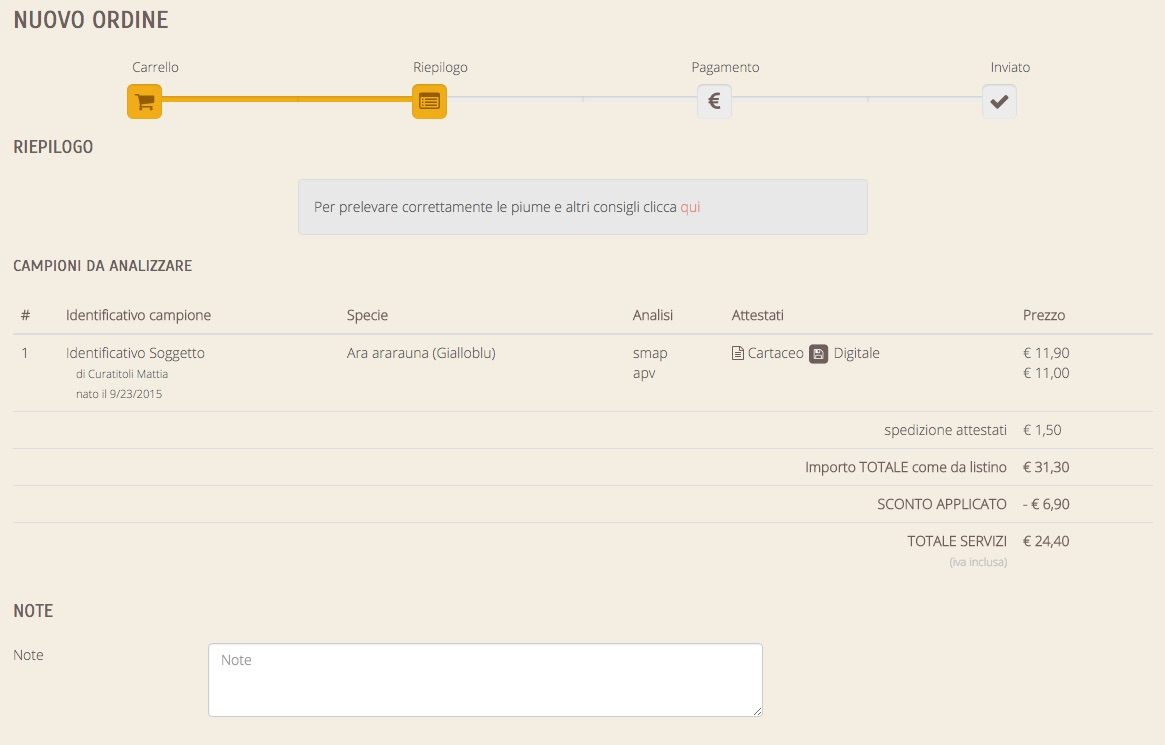
\includegraphics[width=\textwidth]{images/cl-nuovo-ordine-riepilogo} 
   \caption{riepilogo}
   \label{fig:cl-nuovo-ordine-riepilogo}
 \end{subfigure}
 \begin{subfigure}[b]{0.33\textwidth}
   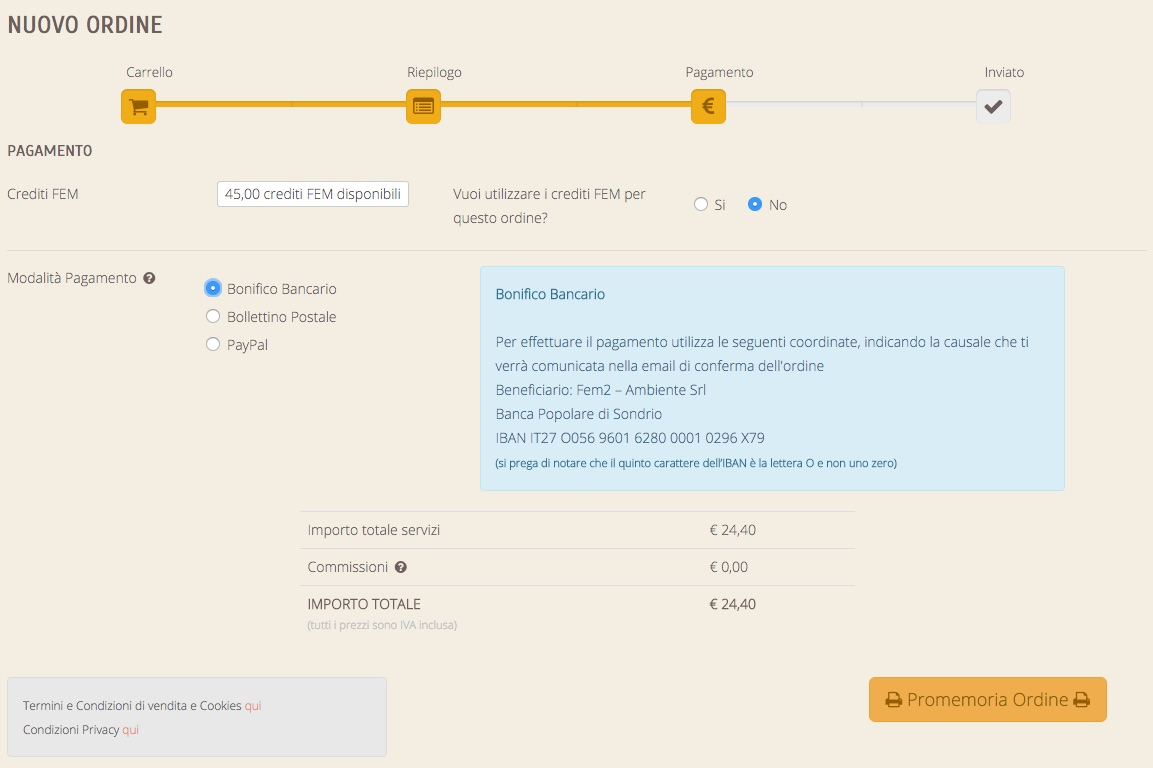
\includegraphics[width=\textwidth]{images/cl-nuovo-ordine-pagamento}
   \caption{pagamento}
   \label{fig:cl-nuovo-ordine-pagamento} 
 \end{subfigure}
 
 \begin{subfigure}[b]{0.6\textwidth}
   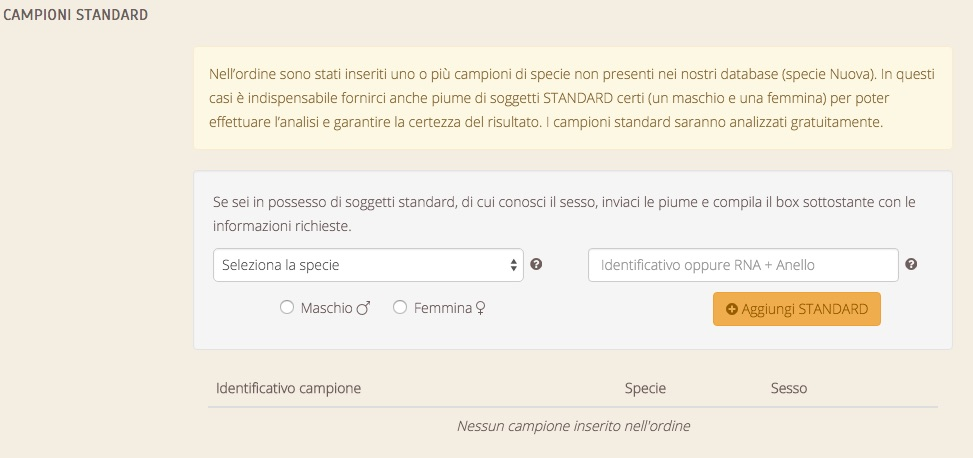
\includegraphics[width=\textwidth]{images/cl-nuovo-ordine-r-standard} 
   \caption{richiesta di standard}
   \label{fig:cl-nuovo-ordine-r-standard}
 \end{subfigure}
 \begin{subfigure}[b]{0.45\textwidth}
   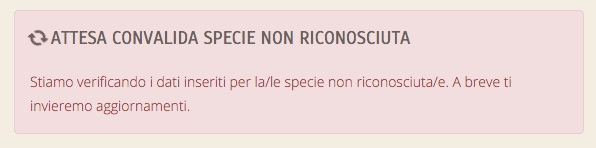
\includegraphics[width=\textwidth]{images/cl-nuovo-ordine-attesa}
   \caption{attesa gestione da parte dei tecnici FEM}
   \label{fig:cl-nuovo-ordine-attesa} 
 \end{subfigure}
 \caption{flusso di creazione nuovo ordine}
\end{figure}

\section*{Ordine}
Una volta creato l'ordine il cliente viene automaticamente indirizzato alla pagina dedicata, accessibile anche attraverso la propria pagina personale.

In questa pagina si trovano tutte le informazioni relative all'ordine suddivise in sezioni:
\begin{itemize}
 \item \textsf{intestazione} con le informazioni chiave dell'ordine, ovvero il numero e lo stato in cui l'ordine si trova;
 \item \textsf{pagamento}: sezione contenente le coordinate per il pagamento visualizzabile solo in caso in cui il pagamento non sia già stato pervenuto;
 \item \textsf{campioni}: tabella con i campioni che riassume tutti i soggetti inseriti da analizzare con a fianco le corrispondenti analisi richieste, lo stato, e l'eventuale presenza di attestati richiesti. In caso di attestati digitali, quando disponibili, il tasto diventa cliccabile è permette il download, in caso di attestati cartacei  invece viene indicato nel tasto quando vengono spediti;
 \item \textsf{comunicazioni}: elenco dei messaggi relativi all'ordine; ad ogni cambio di stato il sistema genera in questa sezione un messaggio di spiegazione (ripetuto tramite email) e permette la comunicazione diretta del cliente con i tecnici di {\fem} attraverso un form testuale.
\end{itemize}

\begin{figure}
 \centering
 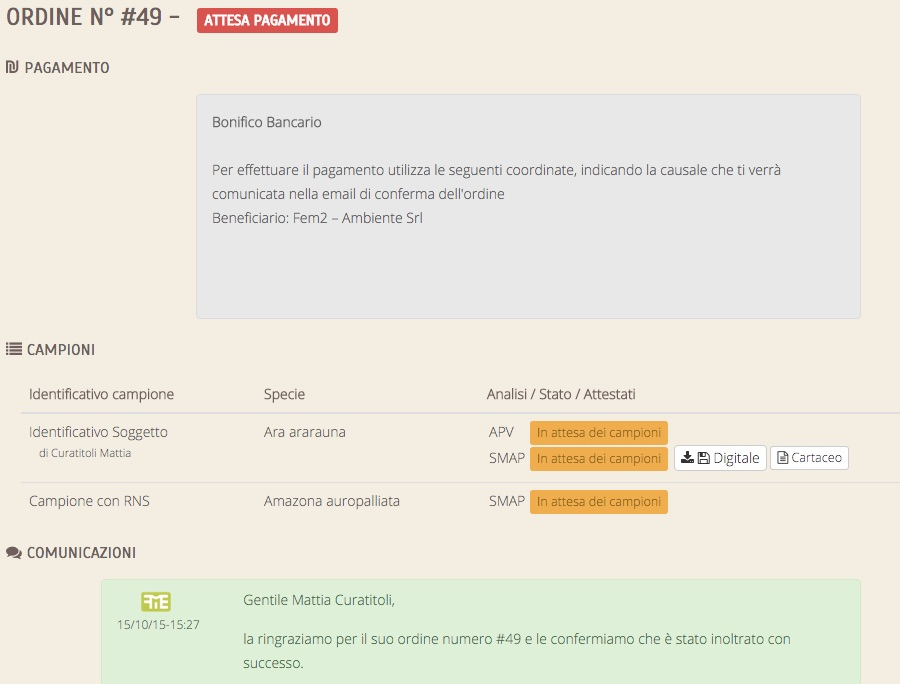
\includegraphics[width=0.8\textwidth]{images/cl-ordine}
 \caption{pagina dell'ordine}
 \label{fig:cl-ordine} 
\end{figure}